% %----------------------------------------------------------------------------------------
% %	PROBLEM 4
% %----------------------------------------------------------------------------------------


\begin{homeworkProblem}[Modèle stochastique]
	
	Dans l’article « Optimising networks Against Malware », l’auteur utilise un modèle
	stochastique basé sur les chaînes de Markov afin de modéliser la propagation d’un vers
	dans un réseau .
	
	\begin{homeworkSection}{4.1}
	
		Expliquez les caractéristiques d’un modèle stochastique et pourquoi ce type de
		modèle s’applique dans le contexte de l’article. Est-ce qu’une approche déterministe
		aurait été préférable? \\
		
		\problemAnswer{
		
		Un modèle stochastique repose sur des variables aléatoires représentant l'évolution possible d'un système au cours du temps. Ce type de modèle s'applique très bien dans le contexte de l'article car on modélise l'évolution de l'infection d'un système de machines au cours du temps, chaque ensemble de machines infectées étant représenté par un état, avec une certaine probabilité \textit{p} de passer à un autre état au temps \textit{t+1} (chaines de Markov).\\
		Une approche déterministe n'aurait pas été réalisable, car les résultats de l'expérience ne sont pas fixes, et donc pas reproductibles. En effet, l'évolution de l'infection dépend de la rapidité à laquelle la première machine infectée réussit à atteindre le \textit{gateway} afin d'atteindre l'autre sous-réseau. Cela se vérifie sur la \ref{ExpG4}, où l'on voit que l'intervalle de confiance de l'expérience est très large.
		
		}
		
		\begin{figure}[h]
			\caption{\label{ExpG4} Expérience avec G=4}
			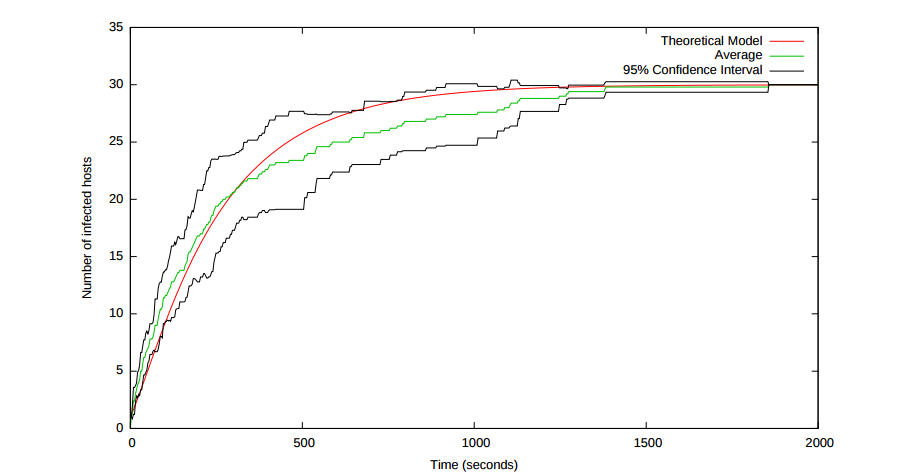
\includegraphics[width=\textwidth]{pictures/results-G=4.png}
		\end{figure}
		
	\end{homeworkSection}

\end{homeworkProblem}

% %----------------------------------------------------------------------------------------
% %	PROBLEM 5
% %----------------------------------------------------------------------------------------

\begin{homeworkProblem}[Performance et optimisation]

	Toujours dans l’article « Optimising networks Against Malware », l’auteur étudie
	l’effet de la topologie du réseau sur la vitesse de propagation d’un vers informatique.\\
	
	\begin{homeworkSection}{5.1}
	
		Appliquez le concept du double-tétraèdre étudié en classe à l’article. Situez votre
		double-tétraèdre dans un contexte d’optimisation, toujours en vous référant à l’article.
		Expliquez quels sont les aspects de votre double-tétraèdre qui sont fixes, et ceux qui sont
		modifiés.\\
		
		\problemAnswer{
			Le double-tétraèdre étudié en classe regroupe les propriétés suivantes :
			\begin{itemize}
				\item L'\textbf{environnement}, commun à l'attaquant et au défenseur
				\item Des \textbf{critères de performance}, propres à l'attaquant et au défenseur
				\item Les \textbf{caractéristiques} de l'attaque et de la défense\\
			\end{itemize}
			
			Les caractéristiques suivantes sont fixées:
			\begin{itemize}
				\item \textbf{Les caractéristiques de l'attaque} : On utilise le \textit{Malware Emulation Framework}, qui produit un ver qui se reproduit en scannant les ip des machines voisines.
				\item \textbf{Les caractéristiques de la défense} : Il n'y en a pas. Dés que l'attaquant scanne l'ip d'une machine, celle-ci est infectée.
				\item \textbf{Le critère de performance de l'attaque} : La vitesse de propagation du virus sur le réseau.
				\item \textbf{Le critère de performance de la défense} : C'est également la vitesse de propagation du virus sur le réseau, mais dans le sens inverse (on souhaite que le virus se propage le plus lentement possible ...)\\
			\end{itemize}
			
			Le seul paramètre variable est l'environnement : on va faire varier la topologie du réseau en jouant sur le nombre de \textit{gateway} interconnectant les différents sous-réseaux.\\
			
			On est donc en présence d'un problème d'optimisation du critère de performance, c'est à dire la vitesse de propagation du ver sur le réseau (qui doit être la plus lente possible du point de vue du défenseur), la variable étant le nombre de \textit{gateway}.
				
		}
		
	\end{homeworkSection}
	
	\begin{homeworkSection}{5.2}
	
		Quels autres aspects/méthodes (autres que la topologie du réseau) pourraient être
		étudiés dans le cadre d’un problème d’optimisation où l’objectif est de limiter la vitesse
		de propagation d’un logiciel malveillant dans un réseau? Donnez au minimum deux
		exemples.\\

		\problemAnswer{
		
			Les autre méthodes suivantes pourraient être étudiées afin de limiter la propagation d'un logiciel malveillant dans le réseau:
			
			\begin{itemize}
				\item L'utilisation d'un \textit{firewall}, filtrant l'utilisation de certains ports, traditionnellement utilisés pour transmettre des virus (telnet, ...)
				\item Le blocage de certains paquets ICMP (comme le \textit{ECHO} utilisé par la commande \textit{Ping}) afin d'empêcher l'attaquant de scanner les ports ouverts d'une machine.
				\item L'utilisation d'un antivirus ayant une base de donnée des signatures des virus connus, ou étant capable de reconnaître les comportements suspects des virus (ouverture de connexion sur des ports peu usités, ...)
				\item Demander à l'utilisateur une confirmation avant l'installation de tout programme en provenance du réseau.
			\end{itemize}
			
		
		}
	
	\end{homeworkSection}
	
	\begin{homeworkSection}{5.3}
		
		Il a été démontré qu’une plus grande biodiversité au sein d’un écosystème permettait
		de ralentir la propagation des virus ou des bactéries dangereuses. Comment pourriez-vous
		appliquer le concept de diversité au sein d’un réseau informatique? Quelle(s) forme(s)
		prendrait cette diversité? \\
		
		\problemAnswer{

		
		}
	
	\end{homeworkSection}


\end{homeworkProblem}